\documentclass{article}

\usepackage[final]{neurips_2022}
\usepackage{graphicx} %package to manage images
\graphicspath{ {./Images/} }
\usepackage[rightcaption]{sidecap}
\usepackage{wrapfig}


\title{Report on Correlation of Pitching Velocity and Injury}


\author{Jack Greff and Jack Sampson \AND CS260 \AND December 15th, 2022 }

\begin{document}
 \LARGE

\maketitle

\section{Introduction and Related Works}

With modern technology and technique advancements in pitching mechanics, pitching velocities have also increased significantly. For example, in the 2008 season, only 196 pitches reached 100mph across the entire season. Yet, consistently, as early as 2015, there have been over 1000 pitches that have reached that threshold \cite{Source3}. As a fan, this may appear great and entertaining, yet the longevity, maintenance, and health of these pitchers remain in question.  As pitchers ourselves, it’s important to educate ourselves about the effects of pushing your body to the limit. The road to recovery from a serious elbow surgery normally takes  1 to 2 years to fully recover, and for a college career, losing this time can be extremely costly. Our method helps educate us in the exact ways that are helpful to us. 

In the past, some sources indicate that pitching velocity is “associated with risk of ulnar collateral ligament (UCL) injury” as a 2016 study in the National Library of Medicine study found \cite{Source2}. On the other hand, a different 2016 study in the National Library of Medicine found that velocity explained less than 7 percent of the variance in UCL reconstruction \cite{Source4}. UCL Reconstruction surgery, commonly known as Tommy John surgery in the baseball world, is the most common serious pitching injury common repairs in the MLB and surgery has been preformed over 1000 times in the MLB \cite{Source1}.  As the relatively recent findings have contradictory reports, we wanted to analyze and create our own data to educate ourselves on the issue. With 2 of the Haverford baseball team’s highest velocity pitchers having undergone Tommy John surgery, the relationship between velocity and injury is equally prevalent to us as it is in the MLB. 

\raggedbottom 
\section{Method}




Our group investigated the correlation between Pitchers average fastball velocity and whether or not they injured their arm in the 2022 MLB season. Specifically, a player qualifies if they were on the 15-day injured list or higher during the regular or postseason. To find this correlation we sampled the 100 hardest throwing MLB pitchers (average fastball velocity) relative to a sample of 100 random Pitchers throwing the MLB average (93mph-94mph). Because we manually entered the information, this was a realistic sample size. Our data was as low as 93.0mph to 100.8mph. The lowest value for the 100 hardest throwers was 96.1 and the highest for the league average throwers was 94.0. Our data was well dispersed and given the limits of our sample size and the objective of our analysis, this collection of data made the most sense. 
    
We mapped the data on a GGplot graph, plotting the probability of arm injury as a function of average pitching velocity  with an average posterior probability of injury line and 95 percent credible intervals. 

.

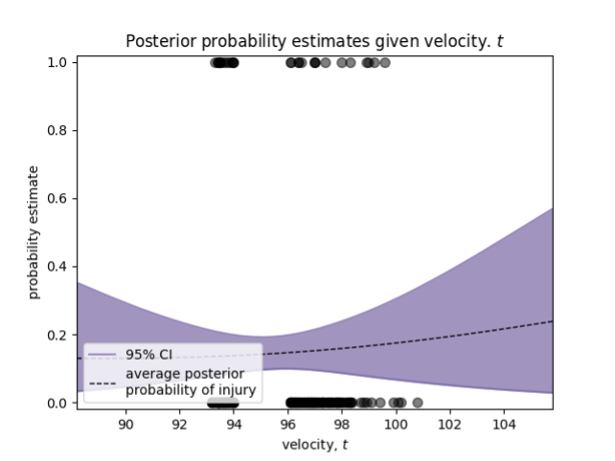
\includegraphics{Graph}

\raggedbottom 
\section{Analysis}

We hypothesized that there will be a clear, well-supported relationship that indicates higher velocities have a higher probability of injury. While the graph shows the average posterior probability of arm injury is slightly increasing and indicates a very slight increase in injury likelihood as velocity increase, the credible intervals and the growth of average probability are not strong enough for a correlation. According to the CI, it's entirely possible for a population to consistently have less likelihood of injury as velocity grows according to our model, which is extremely unlikely in the real world. According to the model, its plausible for the average probability of 90mph to be roughly 30 percent and 100mph to be nearly 10 percent. Because of wide credibility, our model cannot be seriously taken and no statistically relevant correlation can be drawn. 

A major reason a statistically relevant correlation was not found is because of the limitations of our experiment. Because injury data is not readily available and was collected manually, we had to choose to limit the data to the 2022 season. We found that limiting the scope made it harder to find a correlation, as many pitchers in the 100 hardest throwers have had Tommy John surgery or other arm injuries directly related to pitching within the last 5 years. A potential solution would expand the window of injury to 5 years or a longer period of time, but a pitcher who has pitched in the MLB for five seasons is inherently more at risk of injury relative to an MLB rookie. Additionally, there would be no data for rookies in the minor leagues, so that data would be immediately tainted, even though on a year-to-year basis that may not be the case. We expected to see a correlation across the given 2022 season and the data was not able to support this conclusion.

\raggedbottom 
\section{Future Study}

While we cannot conclude a correlation, future experiments could create more conclusive and helpful information. For example, a different model that doesn't operate on a binary scale would distinguish between small injuries and season endings. Bunching injuries together doesn't fully educate us on the health risks of players, as if 95 percent of injuries in our data resulted in Tommy John surgery versus 5 percent of them, for example, our outlook on players' health changes drastically. Ideally, multiple graphs are created that show a varety of factors in the pitcher category. Service time, age, injury past (i.e. pitchers who have already had injuries), and others could provide a bigger, more complete picture. 

\section{Bibliography}
\bibliography{citations.bib}
\bibliographystyle{plain}



\end{document}
